\chapter{Abordagem Proposta}
\label{cp:7_proposta}

Este capítulo possui como objetivo principal apresentar a proposta de pesquisa na qual essa dissertação se embasou, como também a metodologia utilizada para o desenvolvimento da mesma e alguns resultados esperados com este trabalho.

\section{Definição do problema}
\label{def. Problema}

No ramo biométrico, manipular oclusões de objetos ou faces é uma tarefa difícil quando necessitamos realizar o reconhecimento de uma pessoa em um ambiente irrestrito. No estado de arte existem poucos algoritmos responsáveis por tentar lidar e resolver problemáticas como essa \cite{Targino2018_wvc}. 


Essa pequena quantidade de algoritmos ocorre devido as imagens com oclusões serem coletadas em ambientes não colaborativos, em que o usuário não possui a intenção de colaborar expondo sua face frente a uma câmera, além do mais o ambiente não é de certa forma propício para o processo de coleta de dados. A partir disso surge esse problema na biometria, em que esta, deve tentar se adaptar ao contexto e gerar novos métodos que não sejam intrusivos para a coleta dos dados, possibilitando o aparecimento de oclusões parciais, as quais o sistema deve tentar tratar, removendo a parte ocluída, reconstruindo a face e logo em seguida identificando o indivíduo.

Mediante problemáticas como essa, surge a necessidade de técnicas responsáveis por manipular a parte ocluída, visto que a oclusão possibilita quantidades insuficientes e ruidosas de características, resultando em baixas performances alcançadas pelos classificadores. 

Os algoritmos existentes na literatura possuem índice de detecção e reconstrução de oclusão não tão consideráveis, quando comparados aos algoritmos que lidam com a mesma problemática em ambientes controlados. Com isso, o reconhecimento em ambientes com variações de suas condições sejam elas: iluminação, expressão, oclusão e pose, são oportunos a redução da taxa de reconhecimento.

Conforme já mencionado, o reconhecimento facial baseado em faces não ocluídas ainda não apresenta resultados satisfatórios, devido a dificuldade de extração das características essenciais para a identificação do indivíduo. Apresentando uma pequena quantidade de algoritmos na área com tal iniciativa de pesquisa, configurando baixo desenvolvimento nessa área. É interessante perceber que muitos desses algoritmos para detecção de oclusões parciais são específicos para determinado tipo de oclusão, ou ambiente, não existindo uma técnica que se apresente ideal para todos os tipos de oclusões e ambientes.


\section{Hipótese}
A realização de um estudo comparativo envolvendo técnicas presentes na literatura para detecção e reconstrução de oclusões parciais em imagens de face visando o reconhecimento biométrico servirá como um artefato de consulta para pesquisadores da área, possibilitando uma visão holística das principais técnicas de detecção e reconstrução existentes na literatura como também seus eventuais cenários de vantagens e desvantagens.


\section{Proposta}
%Realizar a identificação de usuários com oclusões parciais  é essencial para fins de segurança e aplicação da lei. Conforme mencionado, identificar as pessoas sem a necessidade de qualquer cooperação para a remoção da oclusão, traz grande conveniência e conforto para os usuários em inúmeros cenários. Por outro lado, identificar a presença de oclusões em locais restritos (por exemplo, hospital, área de construção) e revelar a identidade das pessoas nessas áreas garantem a segurança no ambiente. Da mesma forma, a detecção da presença de oclusão pode identificar pessoas suspeitas em certas áreas (por exemplo, estádios de futebol, caixas eletrônicos, lojas, aeroportos)
%e o reconhecimento facial (apesar da presença de oclusão) nessas áreas pode ajudar a polícia a encontrar criminosos / fugitivos. Em suma, o reconhecimento robusto de faces ocluídas parcialmente é muito importante e tem muitos usos potenciais no mundo da vigilância.

A motivação para desenvolvimento dessa pesquisa surge de estudos promissores na área de biometria, alegando-se que a sociedade apresenta necessidades cada vez maiores de tecnologias que favoreçam segurança e bem-estar de toda a população, a partir dessa justificativa, estudos nesse âmbito apresentam viabilidade de aplicações nos mais diversos setores. Essa prerrogativa de detecção de oclusões parciais em imagens da face, surge a partir da demanda de identificação em ambientes que não necessitem da cooperação do usuário para a coleta de dados.%s A oclusão surge diante da não colaboração do usuário para a sua identificação, eis o motivo do alto índice de oclusões parciais em imagens de face em ambientes não controlados.

O foco deste trabalho nessa área surge com iniciativas a reverter as baixas taxas de reconhecimento em ambientes dessa natureza, pela justificativa de que em cenário como esses, que a pessoa não possui a intenção de colaborar para a sua identificação, lidamos com inúmeros tipos de imagens, algumas identificáveis automaticamente, outras não, o foco deste estudo é nas imagens faciais que não são identificáveis automaticamente devido a presença das oclusões.

Há várias técnicas propostas na literatura para detecção e reconstrução de oclusões parciais em imagens de face. No entanto, não há estudos que mencionem quais técnicas são mais adequadas para determinado tipo de oclusão sobre tal ambiente, visto que existem inúmeros tipos de oclusões e ambientes. Logo, pretende-se avaliar o impacto dessas técnicas na detecção e reconstrução de diferentes tipos de oclusões para o reconhecimento biométrico. Como resultado deste estudo, espera-se identificar os principais pós e contras dessas técnicas como também eventuais limitações, e com isso sugerir qual a técnica mais adequada para os mais diversos tipos de oclusões.

A presente proposta apresenta um grau significativo de contribuição em termos gerais, abrangendo o estado de arte, suas técnicas, algoritmos para detecção e reconstrução de oclusões parciais e condições de viabilidade de aplicação, levando em conta as variações de iluminação, pose, expressão e oclusão. Os resultados obtidos com esta pesquisa serão de grande valia para pesquisadores que trabalham nesse âmbito, como também iniciantes que almejam conhecimento holístico do estado de arte para desenvolvimento de futuras pesquisas, de modo a produzir um conhecimento significativo e enriquecimento para o campo da biometria e para os pesquisadores que tentam colaborar no reconhecimento facial independente das condições de coleta dos dados.

Em suma, um estudo comparativo das técnicas para detecção de oclusões parciais e reconstrução de faces pode contribuir significativamente para a área de reconhecimento facial em ambientes não controlados, visto que a comparação envolve análise e síntese de semelhanças, diferenças e padrões entre as técnicas. De acordo com \citeonline{collier1993comparative} o estudo comparativo tem elevado grau de contribuição científico, dado que ele sugere similaridades e contrastes entre os casos, podendo participar da descoberta indutiva de novas hipóteses e posteriormente construção de novas teorias.  

Mediante todo o contexto na figura, \ref{fig:escopo_dissertacao} é apresentado um esquema contendo todo um escopo deste trabalho. Sendo possível visualizar todos os passos necessários para atingir tal objetivo. 

\begin{figure}[H]
\centering
\caption{Esquema proposto nesta dissertação}
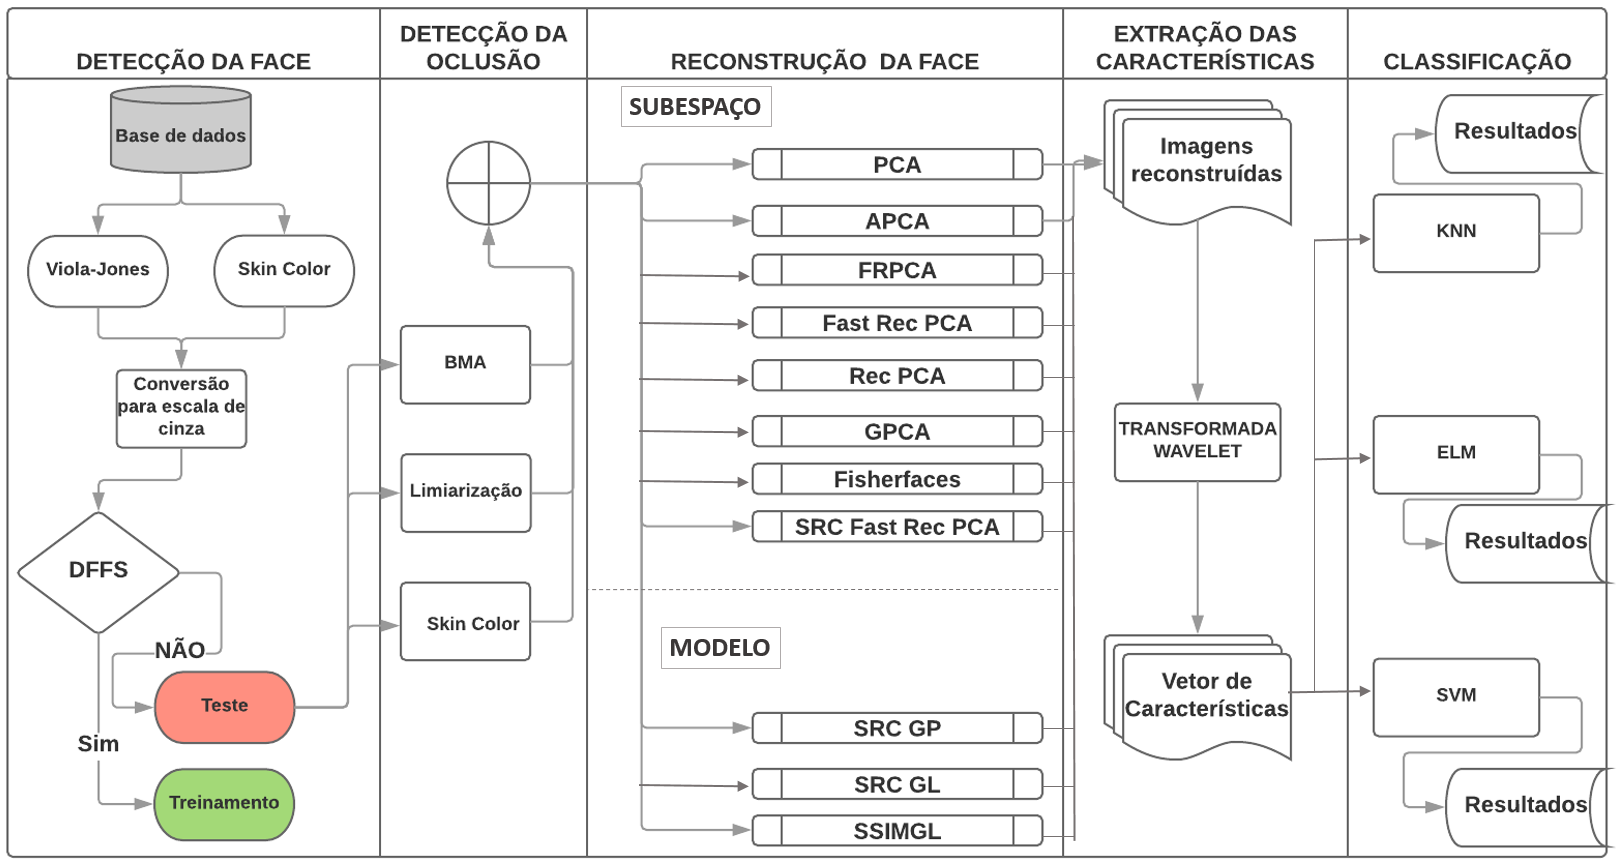
\includegraphics[scale = 0.35]{imgs2/esquema_dissertacao}
\source{Jonas Mendonça Targino, 2018}
\label{fig:escopo_dissertacao}
\end{figure}



\section{Método}

Inicialmente, foi realizada uma RS do estado da arte das técnicas de detecção e reconstrução de oclusões parciais em imagens de face com finalidades biométricas, essa revisão sistemática pode ser visualizada no trabalho \cite{Targino2018_wvc}, paralelamente foram avaliadas quais as bases de dados mais utilizadas. A partir dos resultados obtidos iniciou-se o processo de implementação das técnicas, visto que algumas técnicas não foram replicadas por conter baixa quantidade de informações acerca da técnica, parâmetros e algoritmos, os quais inviabilizaram o processo de replicação.

Inicialmente foram implementadas técnicas de detecção da oclusão baseadas  em limiarização, entretanto, no decorrer dos experimentos verificou-se técnicas mais robustas para detecção da oclusão como o BMA, esta sendo utilizada nos experimentos apresentados neste trabalho. Paralelamente, foram implementadas técnicas de reconstrução de faces parcialmente ocluídas baseadas em subespaço, e logo após partiu-se para as técnicas de reconstrução baseadas em modelo.

Para comparação das técnicas foram utilizadas duas bases de dados de faces parcialmente ocluídas, de modo a possibilitar alguns conjuntos de imagens, visando identificar os prós e os contras de cada técnica como também variações sobre as quais a técnica apresenta limitações (sendo elas: tipos de iluminação, tamanho e forma da oclusão).


Para avaliarmos o comportamento das técnicas de reconstrução e mensurarmos qual técnica apresentou melhores resultados foram utilizadas técnicas de validação da imagem reconstruída como RMSE, SSIM e PSNR. Enquanto outras métricas como taxa de acurácia, matriz de confusão, F1-Score, curvas ROC e curvas de FAR e FRR validaram as técnicas em termos de performance. 

Como técnica de extração de características foi utilizada a Transformada Wavelet utilizando os coeficientes LL nos níveis de decomposição 1, 2 e 3. Enquanto para a tarefa de classificação foram utilizados três diferentes classificadores (K-Vizinhos mais Próximos, Máquina de Aprendizado Extremo e Máquinas de Vetores de Suporte). Teste de significância estatística foram realizados para identificar qual técnica apresentou os melhores resultados perante cada tipo de oclusão.



\section{Proposição de três algoritmos}

Durante a implementação e experimentos das técnicas de reconstrução de faces percebeu-se alguns pontos fortes e fracos de cada técnica. Desta forma, paralelamente ao estudo comparativo foram desenvolvidas três novas técnicas de reconstrução, em que duas delas apresentaram os melhores resultados perante o conjunto de técnicas comparadas neste trabalho. Dessas três técnicas, duas são baseadas em modelo e uma baseada em subespaço. As quais são apresentadas com mais detalhes nas próximas subseções.


\subsection{Representação Esparsa com Fast Recursive PCA}

Essa técnica baseada em subespaço possui um diferencial frente as demais técnicas de mesma natureza, sendo uma análise de representação e classificação da imagem de consulta, e também a redução do números de indivíduos para geração do espaço de faces.

Essa técnica possui como base três etapas, sendo elas: (\textit{i}) aplicação da representação esparsa; (\textit{ii}) mineração das imagens obtidas com a SRC; (\textit{iii}) reconstrução com a técnica Fast Recursive PCA. 

Na primeira etapa desse algoritmo é utilizada a SRC com a formulação proposta por \citeonline{huang2010fast} tomando por base os pixels não ocluídos da imagem parcialmente ocluída, de modo que são analisados os mesmos pixels do conjunto de treinamento. Após esse processo são selecionadas as 20 melhores imagens com maior valor do coeficiente de correlação após o retorno da SRC.


Para o cálculo da SRC adotou-se que $\Upsilon$ é a imagem parcialmente ocluída representada como um sinal, de modo que a matriz de treinamento é da forma $\Gamma$ = $[I_1,I_2,\cdots, I_M]$, contendo $M$ imagens. E $\mathbf{x}$ representa o vetor de coeficientes de correlação. Logo, na equação \ref{eq:SR} é apresentada a estrutura da SRC.

\begin{equation}
y = \alpha_1I_1 + \alpha_2I_2 + \cdots + \alpha_MI_M = \mathbf{\Gamma} \cdot \mathbf{x}
\label{eq:SR}
\end{equation}

O vetor de coeficientes de correlação de forma $\mathbf{x} = [\alpha_1,\alpha_2, \cdots, \alpha_M]$ possuem importância significativa para a imagem parcialmente ocluída, visto que o valor de $\alpha_i$ no intervalo [0,1] representa a semelhança entre as imagens $I_i$ e $y$. Logo, quanto maior o valor de $\alpha_i$ maior sua correlação com a imagem parcialmente ocluída. Dessa forma vetor $\mathbf{x}$ é esparso, ou seja, a maioria de seus valores são próximos de zero. 

Dessa maneira de acordo \citeonline{[32]wright2009robust} apenas as imagens correspondentes aos maiores valores dos coeficientes de correlação apresentam maiores semelhanças perante a imagem de consulta $\Upsilon$. Dessa forma, no contexto de faces parcialmente ocluídas para obtermos valores de alfa com maiores valores de confiança devemos realizar a comparação dos pixels não ocluídos da imagem $\Upsilon$ com os pixels não ocluídos das imagens do conjunto de treinamento $\Gamma$.

Logo a SRC pode ser vista como uma equação linear, da forma $y = \mathbf{\Gamma} \cdot \mathbf{x}$, sujeita ao problema otimização da equação \ref{eq:minsr} .

\begin{equation}
\label{eq:minsr}
(l^1): \hat{x_1} = argmin\left \| x \right \|_1  x \mapsto  \Gamma \cdot \mathbf{x} = y
\end{equation}


Após as 20 melhores imagens selecionadas de acordo com seu coeficiente de correlação, foi utilizada uma zona de pixels de borda da oclusão. Em que essa zona de pixels abrangia um total de 10 pixels, sendo demarcada a partir da aplicação do filtro morfológico de erosão na máscara de oclusão 10 vezes consecutivas.



Enquanto que na etapa 2 para mineração da face com maior semelhança advinda da representação esparsa foi utilizada a técnica SSIM proposta por \citeonline{ssim2004} para análise das similaridades entre os pixels de borda da imagem de consulta e os respectivos pixels das 20 imagens de treinamento provindas do retorno da SRC.

Para a reconstrução da face foi utilizada a técnica Fast Recursive PCA proposta por \citeonline{wang2007reconstruction}, também apresentada neste trabalho.

Na terceira e última etapa é gerado o espaço de faces com todas as imagens de face de três indivíduos, sendo eles:

\begin{itemize}

 \item o primeiro individuo sendo obtido com o maior valor de coeficiente de correlação retornado pela SRC; 
 \item o segundo indivíduo é o que mais se repetiu perante os 20 melhores retornados com a SRC; 
 \item E o terceiro indivíduo é proveniente da etapa de mineração dos dados, sendo o que apresentou maior SSIM dos pixels de borda da oclusão com os respectivos pixels das imagens de treinamento.

\end{itemize}

Na figura \ref{fig:estrutura_src_fast_rec_pca}  podemos visualizar a estrutura como também a sequência dos passos para reconstrução com essa nova técnica.

\begin{figure}[H]
\centering
\caption{Estrutura da técnica SRC com Fast Recursive PCA}
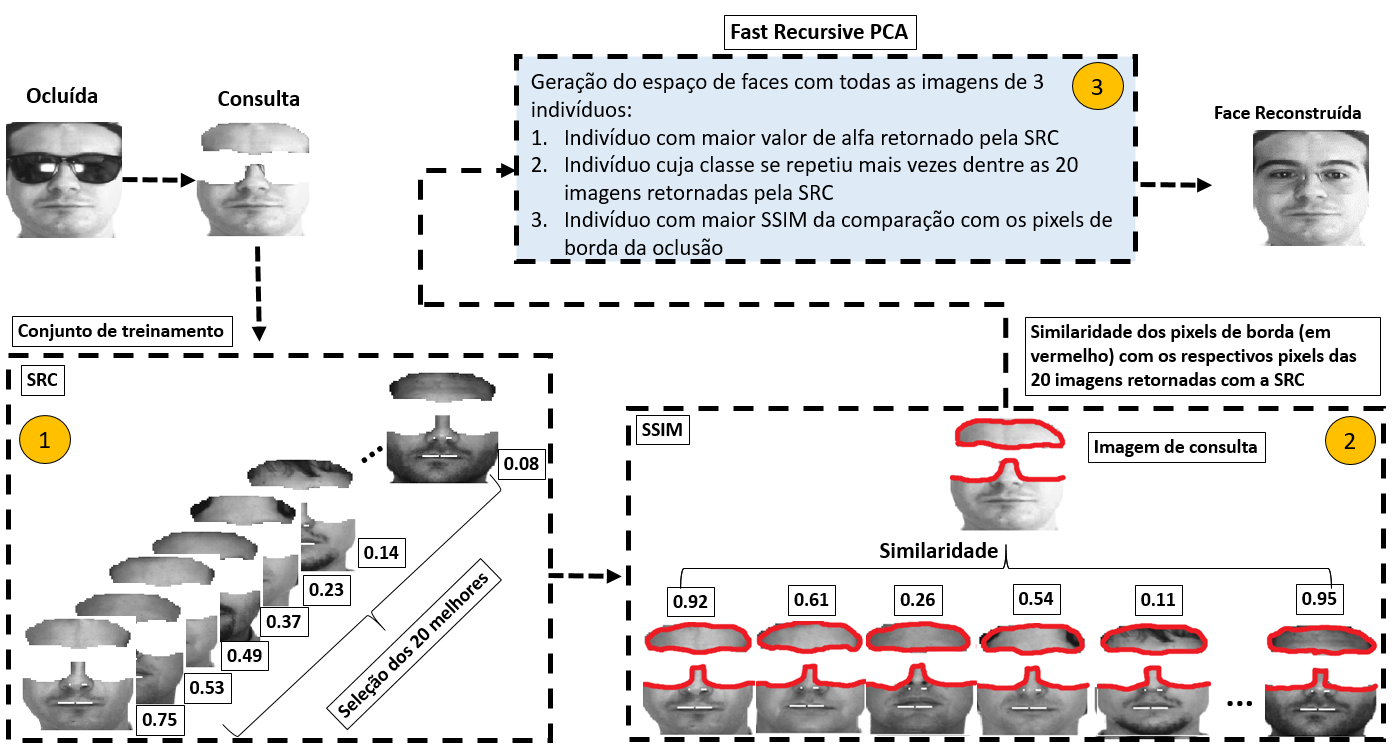
\includegraphics[scale = 0.40]{imgs4/estrutura/estrutura_src_fast_rec_pca}
\source{Jonas Mendonça Targino, 2018}
\label{fig:estrutura_src_fast_rec_pca}
\end{figure}



\subsection{Representação Esparsa com Grafo Laplaciano}
\label{sub:SRC_GL}

Essa técnica aqui proposta possui como princípio geral aplicação da Representação Esparsa para classificação das faces de treinamento com maiores semelhança com a imagem parcialmente ocluída para logo em seguida realizar a reconstrução com grafo Laplaciano.

Essa técnica é constituída de três passos sendo eles: (\textit{i}) aplicação da representação Esparsa com a formulação proposta por \citeonline{huang2010fast} no conjunto de imagens de treinamento; (\textit{ii}) mineração da imagem com maior coeficiente de correlação; (\textit{iii}) reconstrução com grafo Laplaciano.


O primeiro passo dessa técnica possui como objetivo realizar a classificação da face de treinamento com maior proximidade da face parcialmente ocluída. Como entrada para a SRC foram utilizados os pixels não ocluídos da imagem ocluída, dessa forma, a SRC buscava as faces com maiores coeficientes de correlação dos respectivos pixels do conjunto de treinamento. Dessa forma foram selecionadas as 20 imagens do conjunto de treinamento com maiores coeficientes de correlação.

Após o retorno das 20 imagens de face com maiores coeficientes de correlação utilizou-se os pixels vizinhos da oclusão de modo a analisar a similaridade dos pixels vizinhos não ocluídos da imagem ocluída com os respectivos pixels das 20 imagens retornadas. Para geração da borda de oclusão foram utilizados 10 operadores morfológicos de erosão (resultando em uma borda de oclusão com 10 pixels) na máscara de oclusão de modo a identificar os pixels de borda. 

Após os pixels de borda selecionados da imagem de consulta e das 20 imagens de treinamento, foi utilizado o algoritmo KNN com distância Euclidiana de modo a identificar qual a face que possui as regiões de borda dos pixels ocluídos com menor distância (ou seja com maior semelhança dos pixels). Dessa forma a distância do KNN é calculada tomando por base a equação \ref{eq:knn_src_gl}. Em que $J_{I_i}$ e $J_y$ representam respectivamente os pixels de borda $J$ da imagem $I_i$ e da imagem de consulta.

\begin{equation}
Dist = \sqrt{\sum_{i=1}^{n} (J_{I_i} - J_y)^2 }
\label{eq:knn_src_gl}
\end{equation}

Nesse algoritmo, a topologia de conexão de um nó é alterada para os $k$ vizinhos mais próximos, neste caso o $k$ possui valor 10. A figura \ref{fig:topologia_grafo} ilustra a área $J$ dos pixels de borda, como também a topologia do grafo Laplaciano utilizado nesse trabalho, em que o ponto vermelho representa o pixel corrente e todos os outros 10 pontos representam seus 10 pixels vizinhos.


\begin{figure}[H]
\centering
\caption{Topologia do grafo Laplaciano}
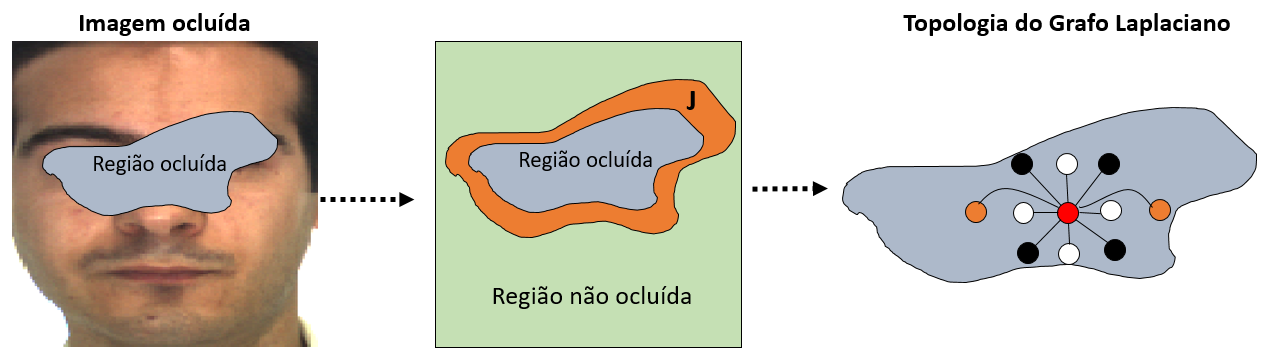
\includegraphics[scale=0.45]{imgs/regiao2.png}
\source{Jonas Mendonça Targino, 2018}
\label{fig:topologia_grafo}
\end{figure}

A formulação matemática dessa técnica difere-se da técnica SRC com grafo de Poisson apresentada na subseção \ref{sub:RS_GP} e proposta por \citeonline{[25]deng2011graph} por utilizar KNN em vez de SSD nos pixels de borda $J$, também por utilizar uma nova topologia com 10 conexões por pixel, e além do mais sua matriz Laplaciana também apresenta modificações quanto ao número de conexões por pixel.

Logo para descobrirmos os pixels que irão ser substituídos pelos pixels ocluídos temos que resolver o sistema que pode ser decomposto com o auxílio da formulação abaixo. É importante notarmos a diferença da matriz Laplaciana na topologia do grafo Laplaciano.

\[
\begin{matrix}

\\
L = D - W \\
L = diag\left [  \sum_{j}W_{ij} \right ] - W\\
\\
= \begin{bmatrix}
\begin{matrix}
\sum_jW_{1j} &    & \\
  &  \sum_jW_{2j} &  & \\
  &  & \ddots & \\
  &          & & \sum_jW_{nj} 
\end{matrix}
\end{bmatrix}

- W
\\[6pt]
\\[6pt]
%\\[6pt]
\textit{Dessa maneira a matriz Laplaciana do grafo com 10 conexões é da forma:} \\[6pt] \\[6pt]


\textbf{L}G_{no}=\begin{bmatrix}
\begin{matrix}
10 &  -1  & -1 &-1 &-1 &\ldots 0\\
-1  &  10 & -1 &-1 &-1 &\ldots  0\\
-1  &-1  & 10   &-1 &-1 &\ldots0\\
-1  &-1  &-1   &10 &-1 &\ldots0\\
\vdots & \vdots & \ddots &  &\ddots\\
0  &   \ldots&-1 & -1 &-1    &10
\end{matrix}
\end{bmatrix}
.
\begin{bmatrix}
\begin{matrix}
G_{no_1} \\
G_{no_2}  \\
G_{no_3} \\
$\vdots$\\
G_{no_{(n-1)}} \\
G_{no_n}  \\
\end{matrix}
\end{bmatrix}
\\%[6pt]
%\\[6pt]
\textit{Com isso, chegamos a resolução do sistema geral, pela forma:} 
\\%[2pt]
%\\
\textbf{L}G_{no} = \kappa\textbf{ L}G{o}
\end{matrix}
\]

 Logo após a descoberta do sistema temos que apenas substituir os pixels ocluídos na imagem parcialmente ocluída pelos pixels retornados pela resolução do sistema linear da matriz laplaciana.



Dessa forma no terceiro e último passo, a imagem correspondente aos pixels de borda com menor distância, ou seja, a imagem $G_{no}$ passada para a reconstrução com grafo Laplaciano. A figura \ref{fig:estrutura_src_gl} ilustra a estrutura da técnica bem como os passos necessários para realizar a reconstrução.


\begin{figure}[H]
\centering
\caption{Estrutura da técnica SRC com Grafo Laplaciano}
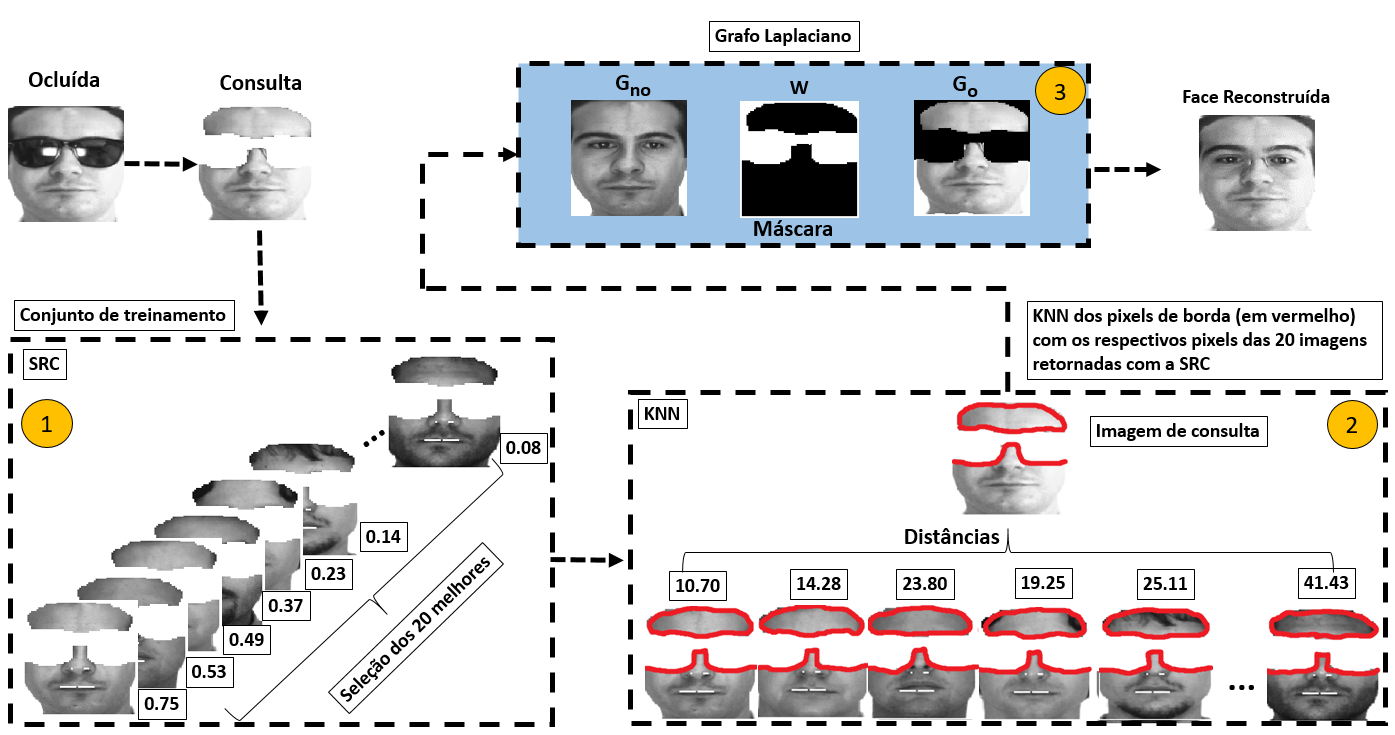
\includegraphics[scale = 0.40]{imgs4/estrutura/estrutura_src_gl}
\source{Jonas Mendonça Targino, 2018}
\label{fig:estrutura_src_gl}
\end{figure}


\subsection{Similaridade Estrutural com grafo Laplaciano}
\label{sec:ssim_gl}


Uma grande quantidade de técnicas para classificação e identificação de faces vem sendo dispostas na literatura, entretanto, essas técnicas apresentam queda de desempenho quando apresentadas a ambientes não controlados, um dos maiores fatores que impactam essa queda é a oclusão. Entretanto manipular a oclusão não é uma tarefa simples, com isso, inúmeras iniciativas vem sendo apresentadas com iniciativas a realizar uma classificação do indivíduo apenas utilizando a parte não ocluída, algumas dessas iniciativas são os trabalhos de \citeonline{[25]deng2011graph},\citeonline{[6]yang2014fast} e \citeonline{[32]wright2009robust} que utilizam SRC. Umas das desvantagens dessas técnicas é que ao lidar com imagens com variações de oclusões e iluminação há queda considerável de performance, sem contar que a SRC em imagens com tais variações necessita de outras técnicas (como SSD, KNN e SSIM) de modo a complementar seu resultado, em alguns trabalhos são utilizadas técnicas baseadas em distância para tentar encontrar as faces do conjunto de treinamento com maiores similaridades.


Essa técnica também construída durante a elaboração deste trabalho, sendo intitulada de SSIMGL. Constitui-se de três passos principais que são: (\textit{i}) redução do tamanho de todas as imagens de modo a reduzir a complexidade do problema; (\textit{ii}) aplicação da técnica de validação de imagens Similaridade Estrutural para classificação da parte não ocluída perante a face parcialmente ocluída; (\textit{iii}) inserção da imagem no grafo Laplaciano no seu tamanho original;(\textit{iv}) aplicação do Grafo Laplaciano para reconstrução da face. 


O primeiro passo dessa técnica possui como base  redução de todas as imagens para a dimensão (32 $\times$ 32) de modo a reduzir o tempo e a complexidade computacional e consequentemente manipular um conjunto de imagens com  menores dimensões. A dimensão (32 $\times$ 32) foi tomada com base em testes realizados, em que visualizou-se que com essa dimensão era possível detectar a parte ocluída de maneira satisfatória e aplicar a similaridade estrutural na parte não ocluída com considerável performance da técnica.

Enquanto a segunda etapa dessa técnica possui como base aplicação da análise da similaridade estrutural \cite{ssim2004} dos pixels não ocluídos da imagem de consulta, com os respectivos pixels das imagens do conjunto de treinamento. A métrica SSIM está descrita com mais detalhes na subseção \ref{sub:ssim}. Nessa etapa o mais importante dela é verificar quais das imagens do conjunto de treinamento possui maior SSIM ao realizar a comparação dos pixels não ocluídos da imagem de consulta com os respectivos pixels da imagem do treinamento.
	


 A métrica SSIM foi escolhida visto que  segundo \citeonline{thung2009survey} essa métrica atua de forma a simular o grau de percepção humana, se ajustando independente do ambiente de coleta da imagem. Portanto, essa métrica possibilita consideráveis resultados independente do ambiente de coleta. 
 
Enquanto o terceiro passo tem como objetivo utilizar a imagem com maior SSIM no seu tamanho original (128 x 128) fornecendo melhor qualidade de reconstrução. Dado que reduzir a dimensão das imagens no primeiro passo é interessante para reduzir o tempo computacional utilizado.

E o último passo e não menos importante dessa técnica é a reconstrução da imagem de consulta com grafo Laplaciano. A reconstrução com grafo Laplaciano possui funcionamento similar ao grafo Laplaciano descrito matematicamente na subseção \ref{sub:RS_GP}, diferenciando-se por utilizar os 10 nós vizinhos para geração do grafo, enquanto no grafo de Poisson são utilizados apenas o 4 vizinhos(acima, abaixo, esquerda e direita), dessa forma, paralelamente alterando a matriz Laplaciana seguindo o modelo matemático do grafo Laplaciano apresentado na subseção \ref{sub:SRC_GL}. O funcionamento e estrutura da técnica SSIMGL é apresentado na figura \ref{fig:estrutura_ssimgl}.



\begin{figure}[H]
\centering
\caption{Estrutura da técnica SSIMGL}
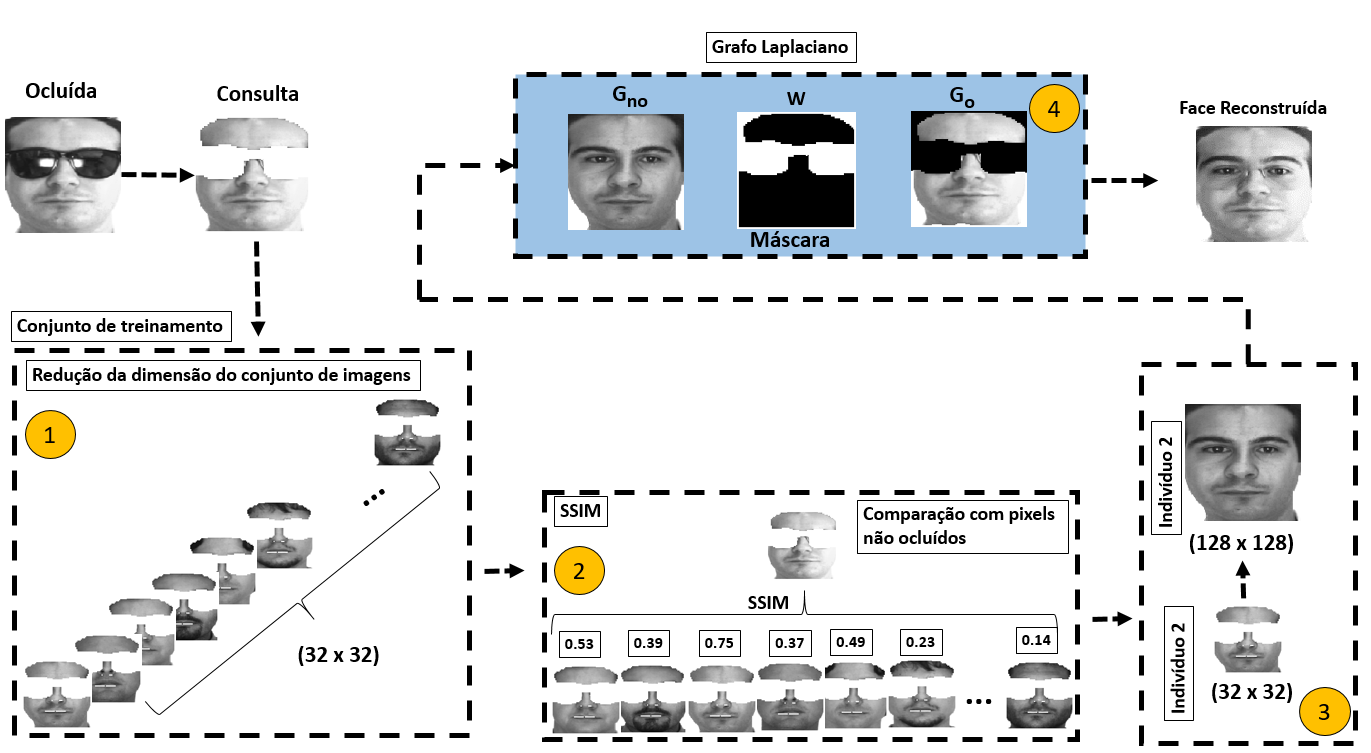
\includegraphics[scale = 0.40]{imgs4/estrutura/estrutura_ssimgl}
\source{Jonas Mendonça Targino, 2018}
\label{fig:estrutura_ssimgl}
\end{figure}


\section{Aplicação no meio científico deste trabalho}

A comparação e proposição de novas técnicas de detecção e reconstrução de oclusões parciais em imagens de face pode produzir novos caminhos e direcionamentos para os pesquisadores da área, dando suporte para a pesquisa e direcionamento holístico do tema de pesquisa e suas consequentes limitações. Além disso, este documento contém uma descrição detalhada e unificada de cada técnica de detecção e reconstrução de imagens de face parcialmente ocluídas. Além de disponibilizar os códigos  de todas as técnicas bem como ilustrações durante a descrição da técnica que ajudam a compreender o funcionamento da mesma.


Acreditamos que este trabalho acarretará em uma contribuição significativa para a área de reconhecimento biométrico, mais especificamente ao reconhecimento facial em ambientes não controlados. Uma outra contribuição deste trabalho é possibilitar subsídios junto a comunidade científica na produção e disponibilização das técnicas de detecção e reconstrução de oclusões parciais em imagens da face, e consequentemente disponibilização das formulações matemáticas de cada algoritmo e seu respectivo código fonte. Objetivando futuras replicações pelos pesquisadores da área e leigos que possuem interesse em se aprofundar no assunto.


\section{Considerações finais do capítulo}

Neste capítulo foram apresentados o problema de pesquisa, a hipótese que este estudo tenta confirmar, a abordagem proposta neste trabalho que é o estudo comparativo das técnicas de detecção e reconstrução de oclusões parciais em imagens de face, bem como também a proposição de três novas técnicas (uma baseada em subespaço e duas baseadas em modelo) as quais espera-se contribuir junto ao meio científico.